\documentclass[a4paper,14pt]{extreport}
  \usepackage[left=1.5cm,right=1.5cm,
      top=1.5cm,bottom=2cm,bindingoffset=0cm]{geometry}
  \usepackage{scrextend}
  \usepackage[T1,T2A]{fontenc}
  \usepackage[utf8]{inputenc}
  \usepackage[english,russian,ukrainian]{babel}
  \linespread{1.5}
  \usepackage{tabularx}
  \usepackage{amssymb}
  \usepackage{color}
  \usepackage{amsmath}
  \usepackage{mathrsfs}
  \usepackage{listings}
  \usepackage{graphicx}
  \graphicspath{ {./images/} }
  \usepackage{lipsum}
  \usepackage{xcolor}
  \usepackage{hyperref}
  \usepackage{tcolorbox}
  \usepackage{tikz}
  \usepackage[framemethod=TikZ]{mdframed}
  \usepackage{wrapfig,boxedminipage,lipsum}
  \mdfdefinestyle{MyFrame}{%
  linecolor=blue,outerlinewidth=2pt,roundcorner=20pt,innertopmargin=\baselineskip,innerbottommargin=\baselineskip,innerrightmargin=20pt,innerleftmargin=20pt,backgroundcolor=gray!50!white}
   \usepackage{csvsimple}
   \usepackage{supertabular}
  \usepackage{pdflscape}
  \usepackage{fancyvrb}
  %\usepackage{comment}
  \usepackage{array,tabularx}
  \usepackage{colortbl}
  \usepackage{fp}

  \usepackage{varwidth}
  \tcbuselibrary{skins}
  \usepackage{fancybox}


  \usepackage{tikz}
  \usepackage[framemethod=TikZ]{mdframed}
  \usepackage{xcolor}
  \usetikzlibrary{calc}
  \makeatletter
  \newlength{\mylength}
  \xdef\CircleFactor{1.1}
  \setlength\mylength{\dimexpr\f@size pt}
  \newsavebox{\mybox}
  \newcommand*\circled[2][draw=blue]{\savebox\mybox{\vbox{\vphantom{WL1/}#1}}\setlength\mylength{\dimexpr\CircleFactor\dimexpr\ht\mybox+\dp\mybox\relax\relax}\tikzset{mystyle/.style={circle,#1,minimum height={\mylength}}}
  \tikz[baseline=(char.base)]
  \node[mystyle] (char) {#2};}
  \makeatother

  \definecolor{ggreen}{rgb}{0.4,1,0}
  \definecolor{rred}{rgb}{1,0.1,0.1}
  \definecolor{amber}{rgb}{1.0, 0.75, 0.0}
  \definecolor{babyblue}{rgb}{0.54, 0.81, 0.94}
  \definecolor{amethyst}{rgb}{0.6, 0.4, 0.8}

  \usepackage{float}
  \usepackage{wrapfig}
  \usepackage{framed}
  %for nice Code{
  \lstdefinestyle{customc}{
    belowcaptionskip=1\baselineskip,
    breaklines=true,
    frame=L,
    xleftmargin=\parindent,
    language=C,
    showstringspaces=false,
    basicstyle=\small\ttfamily,
    keywordstyle=\bfseries\color{green!40!black},
    commentstyle=\itshape\color{purple!40!black},
    identifierstyle=\color{blue},
    stringstyle=\color{orange},
  }
  \lstset{escapechar=@,style=customc}
%}


\begin{document}
\renewcommand{\bibname}{Список використаної літератури}
\pagecolor{white}

%----------------------------------------1
\newtcbox{\xmybox}[1][red]{on line, arc=7pt,colback=#1!10!white,colframe=#1!50!black, before upper={\rule[-3pt]{0pt}{10pt}},boxrule=1pt, boxsep=0pt,left=6pt,right=6pt,top=2pt,bottom=2pt}



\begin{titlepage}
  \begin{center}
  \large
  Національний технічний університет України \\ "Київський політехнічний інститут імені Ігоря Сікорського"


  Факультет Електроніки

  Кафедра мікроелектроніки
  \vfill

  \textsc{ЗВІТ}\\

  {\Large Про виконання курсової роботи \\
  з дисципліни: «Твердотільна електроніка-2»\\[1cm]

  Варіант №22


  }
  \bigskip
  \end{center}
  \vfill

  \newlength{\ML}
  \settowidth{\ML}{«\underline{\hspace{0.4cm}}» \underline{\hspace{2cm}}}
  \hfill
  \begin{minipage}{1\textwidth}
  Виконавець:\\
  Студент 3-го курсу \hspace{4cm} $\underset{\text{(підпис)}}{\underline{\hspace{0.2\textwidth}}}$  \hspace{1cm}Б.\,В.~Лищенко\\
  \vspace{1cm}

  Превірив: \hspace{6.1cm} $\underset{\text{(підпис)}}{\underline{\hspace{0.2\textwidth}}}$  \hspace{1cm}Л.\,М.~Королевич\\

  \end{minipage}

  \vfill

  \begin{center}
  2021
  \end{center}
\end{titlepage}
%-------------------------------------------------------------------------------------------------------------------------------------------------------------
\tableofcontents
%-------------------------------------------------------------------------------------------------------------------------------------------------------------
\newpage
\setcounter{page}{1}

\newpage
\chapter{ВСТУП}

\newpage
\chapter{ТЕХНІЧНЕ ЗАВДАННЯ НА ПРОЕКТУВАННЯ}

\begin{enumerate}
  \item Розробити схему електричну принципову мікросхеми на основі прототипу вказаного за варіантом.
    \item Побудувати таблицю істинності та визначити логічну функцію, яку виконує мікросхема.
    \item Розрахувати порогові напруги транзисторів мікросхеми.
   \item Розрахувати геометричні розміри транзисторів.
    \item Розрахувати геометричні розміри елементів пристрою захисту.
    \item Запропонувати і описати технологію виготовлення мікросхеми, що проектується.
    \item Побудувати топологічне креслення мікросхеми що проектується.
    \item На кресленні топології надати переріз одного з спроектованих транзисторів (за вибором студента) який повністю демонструю всі шари які є в мікросхемі.
    \item Надати креслення всіх, необхідних для запропонованої технології, фотошаблонів. На цих кресленнях позначити штриховкою непрозорі області фотошаблонів.
\end{enumerate}

\newpage
\chapter{АНАЛІЗ СХЕМИ}
%//////////////////
%////   1     ////
%////////////////

  \begin{figure}[h!]
  \center{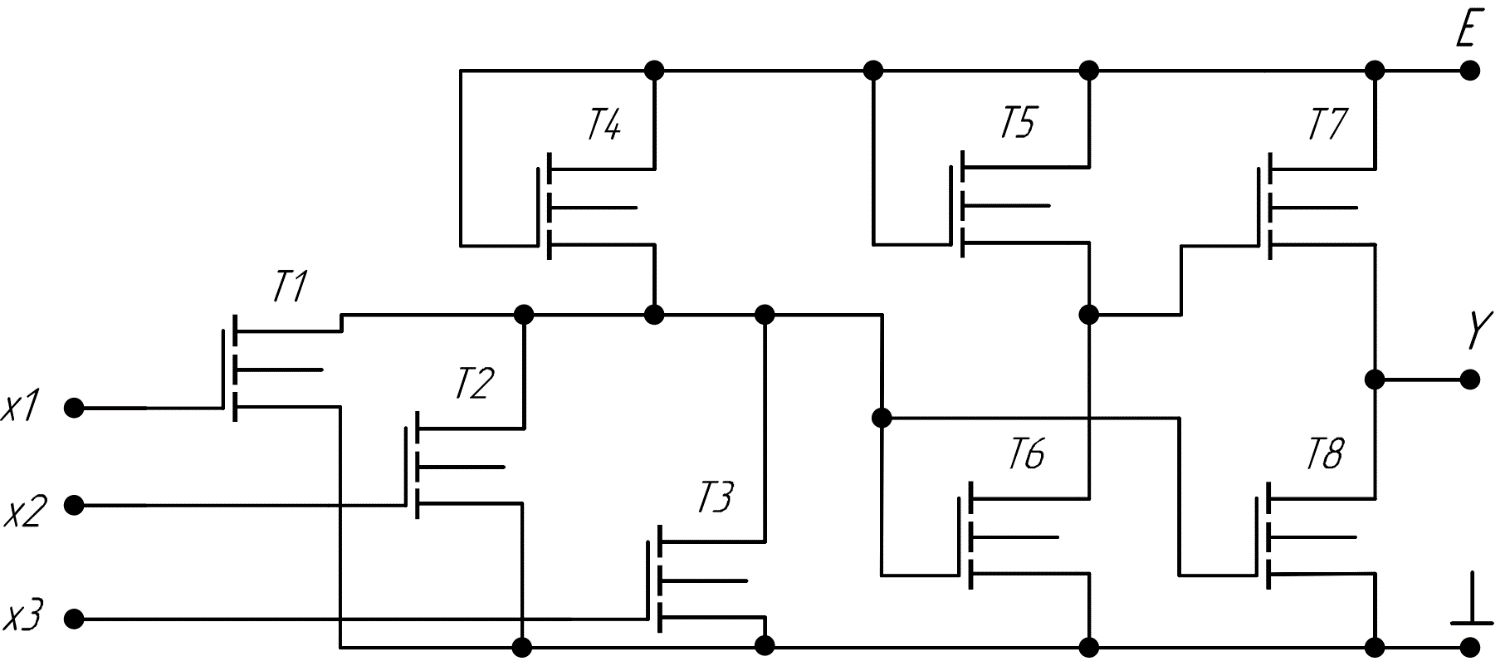
\includegraphics[width=1\linewidth]{1-a.png}}
  \caption{Прототип схеми.}
  \label{ris1}
  \end{figure}
  У мене за варіантом тип підкладки КЕФ, тобто n-тип підкладки, тоді і p-канал у транзисторах.\\

  Тоді, можемо побудувати уже електричну схему на основі прототипу:
  \begin{figure}[h!]
  \center{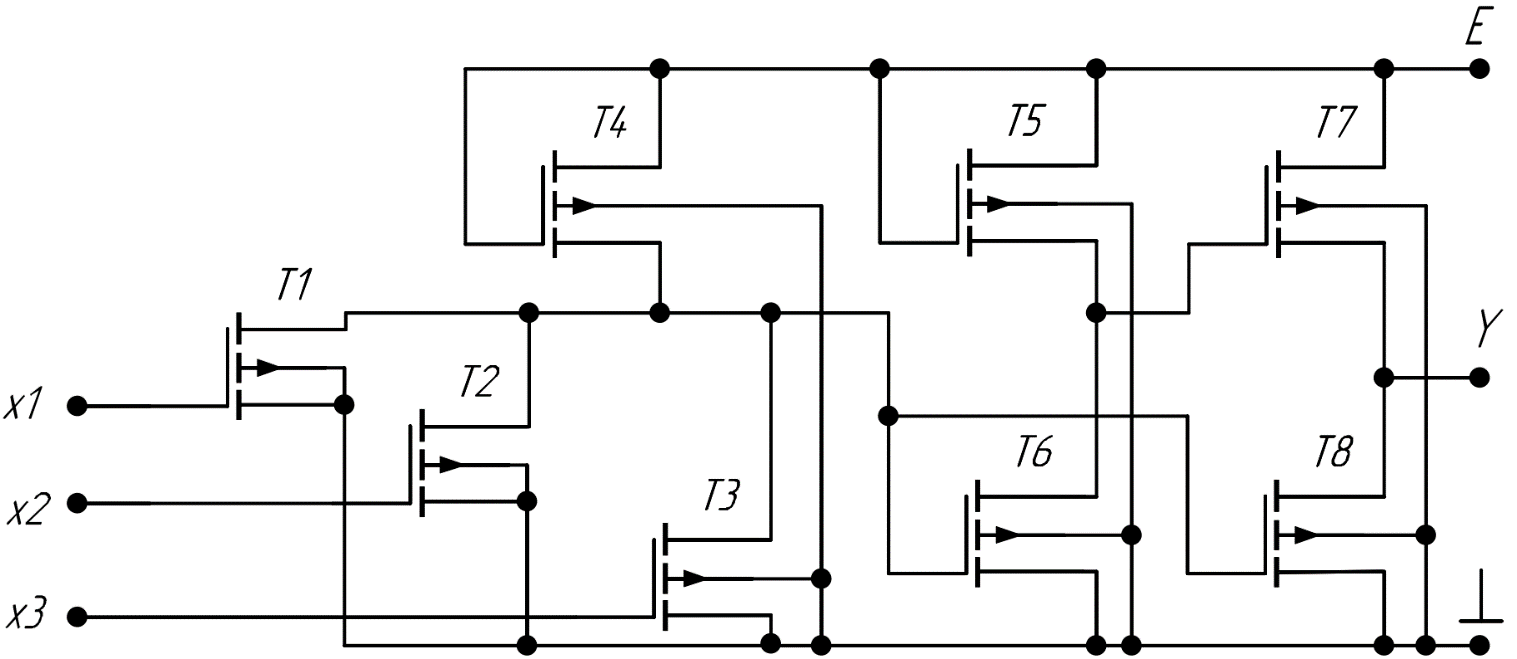
\includegraphics[width=1\linewidth]{2-a.png}}
  \caption{Електрична схема на основі прототипу.}
  \label{ris2}
  \end{figure}
  Так як у нас інтегральна мікросхема, то треба аби всі підклади були підключені до спільного виводу.\\
  \newpage
  Далі переходимо до наступного завдання. Треба скласти таблицю істинності, але легше зробити розбивши схему на каскади. Розглядати будемо спрощену модель схеми, замінивши усі транзистори змінними резисторами, окрім T4 I T5. Так як у них затвор під’єднаний до стоку, то ці транзистори будуть грати роль навантаження, тобто заміняємо їх звичайним резистором. Тоді, спрощена модель:
  \begin{figure}[h!]
    \begin{center}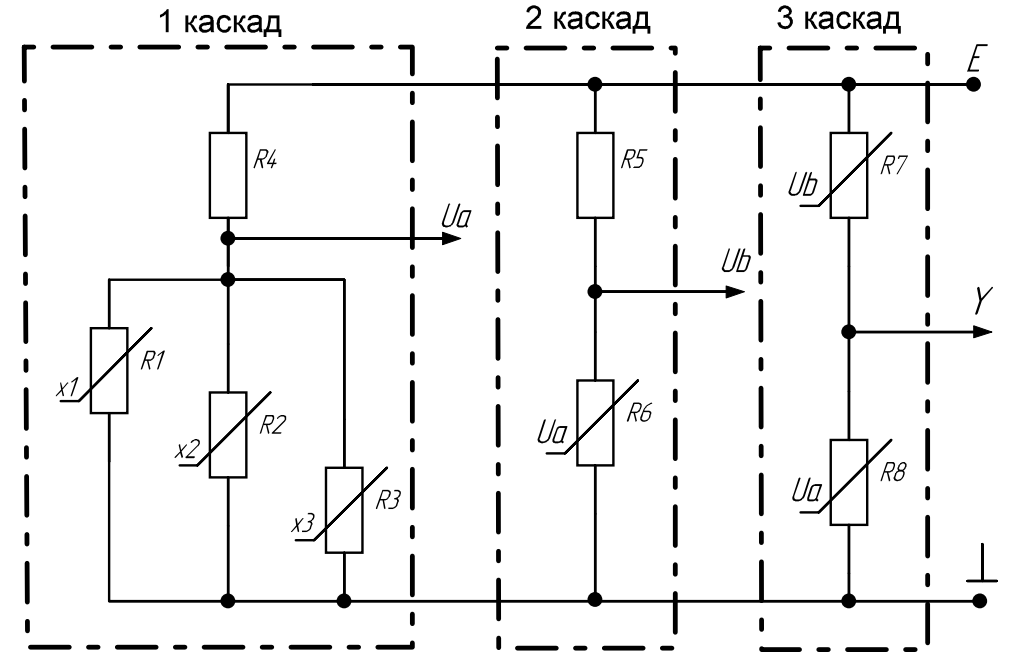
\includegraphics[width=0.7\linewidth]{3-a.png}\end{center}
    \caption{Спрощена модель.}
    \label{ris3}
  \end{figure}


  Бачимо, що у цій схемі всього три каскади. Розпочнемо з першого. У нас три змінних резистори, які можна об’єднати в один ($R_1, R_2$ і $R_3$, так як паралельно підключені). Це виглядатиме так:
  \begin{figure}[h!]
    \center{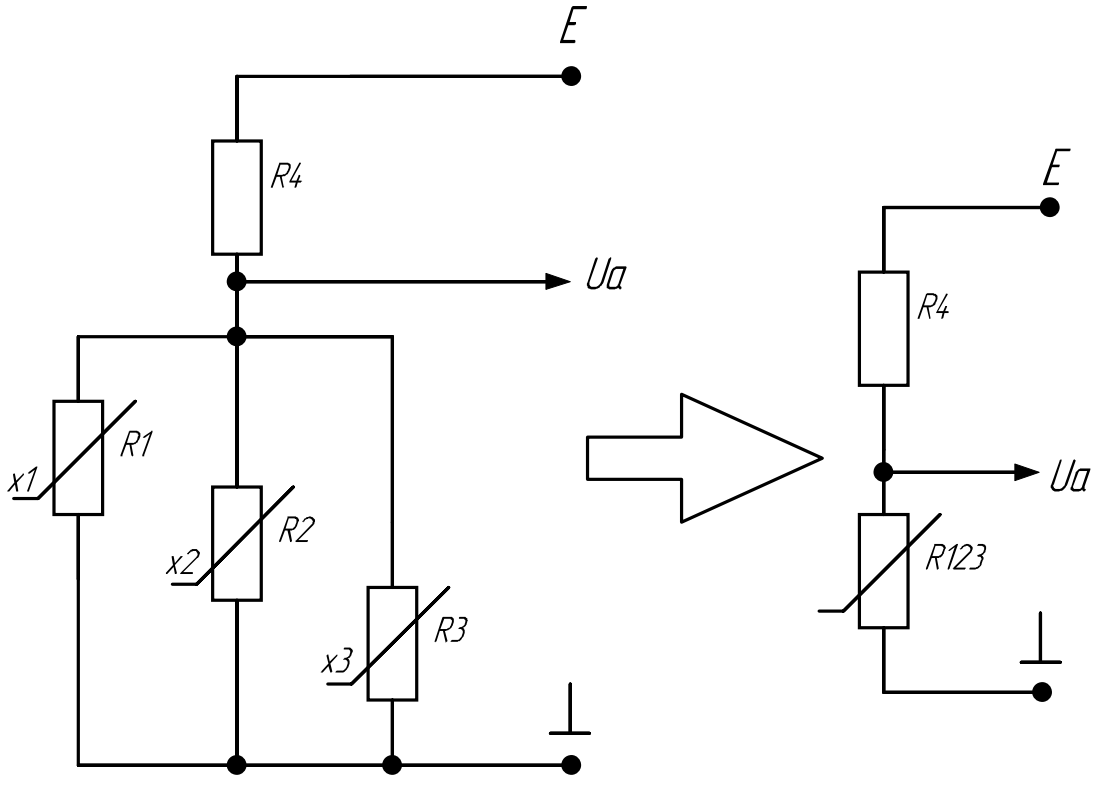
\includegraphics[width=0.6\linewidth]{4-a.png}}
    \label{ris4}
  \end{figure}


  \begin{align}
    \dfrac{1}{R_{123}} = \dfrac{1}{R_{1}}+\dfrac{1}{R_{2}} + \dfrac{1}{R_3};\\
    R_{123} = \dfrac{1}{\dfrac{1}{R_{1}}+\dfrac{1}{R_{2}} + \dfrac{1}{R_3}};
  \end{align}


  \clearpage
  По нашому скороченню, у нас вийшов резистивний дільник напруги (по резисторам $R_{4}$ i $R_{123}$). Знаходимо напругу $U_a$.

  \begin{align}
    U_a = \dfrac{R_{123}}{R_{4} + R_{123}} \cdot E
  \end{align}
  По цих формулах уже можемо складати таблицю істинності для першого каскаду. Так як функція не є складною, можна одразу підставляти числа і шукати опір $R_{123}$.

  \begin{table}[h]
  \caption{Таблиця опорів}
    \begin{center}
      \begin{tabular}{|c|c|c|c|c|c|c|c|c|}
      \hline
      $R_1 $  & 1 & 1 & 1 & 1 & 0 & 0 & 0 & 0 \\ \hline
      $R_2 $  & 1 & 1 & 0 & 0 & 1 & 1 & 0 & 0 \\ \hline
      $R_3 $  & 1 & 0 & 1 & 0 & 1 & 0 & 1 & 0 \\ \hline
  $R_{123} $  & 1 & 0 & 0 & 0 & 0 & 0 & 0 & 0\\ \hline
      %$U_a  $ & 0 & 0 & 0 & 0 \\ \hline
      \end{tabular}
    \end{center}
  \end{table}

  1 – Це коли опір у нас наближається до нескінченності (якщо говорити за опори),а для напруг – коли вона більша за порогову напругу (коли транзистор відкритий), а 0 – це звичайний нуль, коли опір = 0, а напруга менша за порогову напругу. І підставляємо значення резисторів аби знайти Ua.\\

  Тоді, загальна таблиця разом з x1, x2, x3 матиме вигляд:

  \begin{table}[h]
  \caption{Загальна таблиця опорів}
    \begin{center}
      \begin{tabular}{|c|c|c|c|c|c|c|c|c|}
      \hline
      $R_1 $  & 0 & 0 & 0 & 0 & 1 & 1 & 1 & 1   \\ \hline
      $R_2 $  & 0 & 0 & 1 & 1 & 0 & 0 & 1 & 1 \\ \hline
      $R_3 $  & 0 & 1 & 0 & 1 & 0 & 1 & 0 & 1 \\ \hline
      $U_a $  & 1 & 0 & 0 & 0 & 0 & 0 & 0 & 0\\ \hline
      \end{tabular}
    \end{center}
  \end{table}
  Усе, таблиця істинності 1 каскаду зроблена. Далі переходимо до 2 і 3 каскаду:\\
  \begin{figure}[h!]
  \center{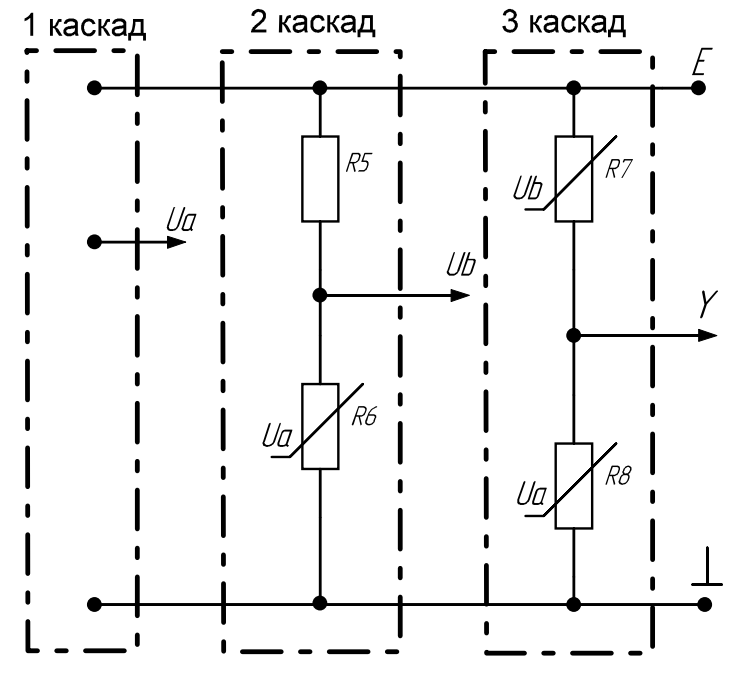
\includegraphics[width=0.5\linewidth]{5-a.png}}
  \label{ris5}
  \end{figure}

  Тут два дільники напруги (2 і 3 каскад відповідно). Можемо одразу скласти формули напруги для Ub та Y:
  $$ U_b = E\cdot \dfrac{R_6}{R_5+R_6}$$
  $$ y = E\cdot \dfrac{R_s}{R_7+R_8}$$

  Складаємо таблицю істинності одразу для двох каскадів:

  \begin{table}[h]
    \begin{center}
    \begin{tabular}{|c|c|c|}
    \hline
    Ua & 1 & 0 \\ \hline
    R6 & 0 & 1 \\ \hline
    Ub & 0 & 1 \\ \hline
    R7 & 1 & 0 \\ \hline
    R8 & 0 & 1 \\ \hline
    Y  & 0 & 1 \\ \hline
    \end{tabular}
    \end{center}
  \end{table}

  Таблиця істинності 2 і 3 каскаду є. Тепер об’єднаємо таблиці істинності першого і другого – третього каскадів:


  \begin{table}[h]
    \begin{center}
  \begin{tabular}{|c|c|c|c|c|c|c|c|c|}
  \hline
  X1 & 0 & 0 & 0 & 0 & 1 & 1 & 1 & 1 \\ \hline
  X2 & 0 & 0 & 1 & 1 & 0 & 0 & 1 & 1 \\ \hline
  X3 & 0 & 1 & 0 & 1 & 0 & 1 & 0 & 1 \\ \hline
  Ua & 1 & 0 & 0 & 0 & 0 & 0 & 0 & 0 \\ \hline
  Ub & 0 & 1 & 1 & 1 & 1 & 1 & 1 & 1 \\ \hline
  Y  & 0 & 1 & 1 & 1 & 1 & 1 & 1 & 1 \\ \hline
  \end{tabular}
    \end{center}
  \end{table}

  Ми побачили, що другий каскад інвертуючий, через що Ub має протилежні знаки відносно Ua, а третій каскад не є інвертуючим, тому і має те саме, що Ub.
  Далі складаємо логічну функцію по отриманій таблиці:
  \begin{equation}
  \begin{array}{c}
  Y=\bar{x}_{1} \cdot \bar{x}_{2} \cdot x_{3}+\bar{x}_{1} \cdot x_{2} \cdot \bar{x}_{3}+\bar{x}_{1} \cdot x_{2} \cdot x_{3}+x_{1} \cdot \bar{x}_{2} \cdot \bar{x}_{3}+ \\
  +x_{1} \cdot \bar{x}_{2} \cdot x_{3}+x_{1} \cdot x_{2} \cdot \bar{x}_{3}+\bar{x}_{1} \cdot \bar{x}_{2} \cdot \bar{x}_{3}= \\
  =\bar{x}_{1} \cdot \bar{x}_{2} \cdot\left(x_{3}+\bar{x}_{3}\right)+\bar{x}_{1} \cdot x_{2} \cdot\left(\bar{x}_{3}+x_{3}\right)+x_{1} \cdot \bar{x}_{2} \cdot\left(\bar{x}_{3}+x_{3}\right)+x_{1} \cdot x_{2} \cdot \bar{x}_{3}= \\
  =\bar{x}_{1} \cdot \bar{x}_{2}+\bar{x}_{1} \cdot x_{2}+x_{1} \cdot \bar{x}_{2}+x_{1} \cdot x_{2} \cdot \bar{x}_{3}=\\
  \bar{x}_{1} \cdot\left(\bar{x}_{2}+x_{2}\right)+x_{1} \cdot\left(\bar{x}_{2}+x_{2} \cdot \bar{x}_{3}\right)= \\
  =\bar{x}_{1}+\bar{x}_{2}+\bar{x}_{3}=\overline{x_{1} \cdot x_{2} \cdot x_{3}}
  \end{array}
  \end{equation}



  І далі, останній крок, малюємо логічну схему по формулі:


  \begin{figure}[h!]
  \center{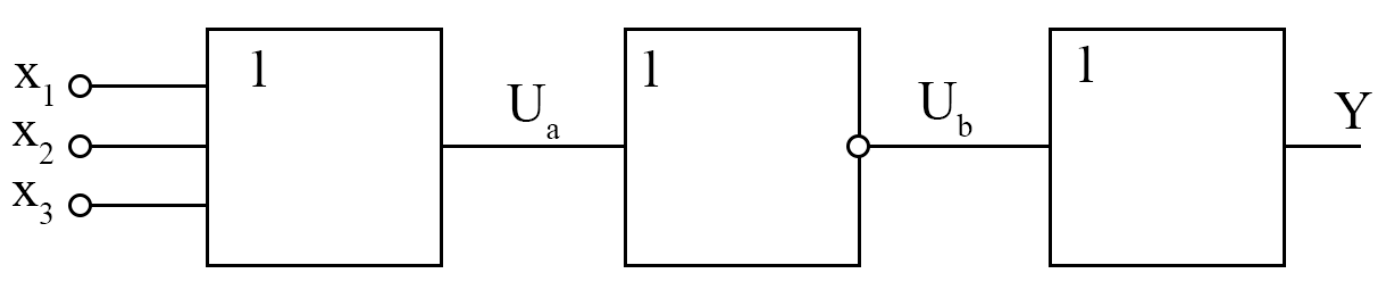
\includegraphics[width=0.9\linewidth]{6-a.png}}
  \label{ris6}
  \end{figure}

\newpage
\chapter{РОЗРАХУНОК ПОРОГОВОЇ НАПРУГИ ІНТЕГРАЛЬНИХ КОМПОНЕНТІВ СХЕМИ}
%//////////////////
%////   2     ////
%////////////////
  Треба записати формулу для пошуку порогової напруги. За варіантом  у мене КЕФ, тому формула буде наступною:
  \begin{equation}
  U_{n o p}^{0}=\phi_{M S}-\dfrac{q \cdot N_{S S}}{C_{o x}}-2 \cdot \phi_{F}-\dfrac{\sqrt{2 \cdot q \cdot \varepsilon_{0} \cdot \varepsilon_{S} \cdot N_{B}}}{C_{o x}} \cdot \sqrt{\left|2 \cdot \phi_{F}+U_{n}\right|}
  \end{equation}

  У цій формулі
  дано майже все, а точніше: $\quad N_{S S}=5,6 \cdot 10^{11} \text{см}^{-3}$
  $\varepsilon_{0}=8,85 \cdot 10^{-14} \text{ }\Phi / \text{см}$
  $q=1,6 \cdot 10^{-19}\text{Кл}$
  $k_{B}=1,38 \cdot 10^{-23}$ Дж/К $, T=300 K,$ $ n_{i}=1,45 \cdot 10^{10} \\
  \text{см}^{-3},$ $ \varepsilon_{S}=11.8,$ $ \rho = 3$  Ом$\cdot$м, $U_0 = -0,6 $ B, $U_1 = -0,6 $ B, $\mu_n = 1500 \text{ }\dfrac{\text{см}^2}{B \cdot c}$


  Питома ємність шукається як
  \begin{equation}
  C_{o x}=\varepsilon_{0} \cdot \varepsilon_{o x} / d_{o x}=\dfrac{8,85 \cdot 10^{-14} \cdot 3,9}{0,5\cdot 10^{-5}}=6,903 \cdot 10^{-8}\text{ } \dfrac{\Phi}{\text{см}^{2}}
  \end{equation}

  Рівень Фермі у об'ємі кремнію:
  \begin{equation}
  \phi_{F}=\left(\dfrac{k_{B} \cdot T}{q}\right) \cdot \ln \left(\dfrac{N_{B}}{n_{i}}\right)
  \end{equation}




  \vspace{0.5 cm}
  $\sigma=\dfrac{1}{\rho}=q \cdot  N_{B} \cdot \mu_{n} \Rightarrow  N_{B}=\dfrac{1}{\rho \cdot q \cdot \mu_{n}}=\dfrac{1}{3 \cdot 1,6 \cdot 10^{-19} \cdot 1500} = 1,39 \cdot 10^{15} \text{ }$ см $^{-3}$
  \vspace{0.5 cm}


  Рівень Фермі тоді буде:
  $$\phi_{F}=\left(\dfrac{k_{B} \cdot T}{q}\right) \cdot \ln \left(\dfrac{N_{B}}{n_{i}}\right)=\dfrac{1,38 \cdot 10^{-23} \cdot 300}{1,6 \cdot 10^{-19}} \cdot \ln \left(\dfrac{1,39 \cdot 10^{15}}{1,45 \cdot 10^{10}}\right)=0,297\text{ } B$$\\

  Напруги між витоком і підкладкою для кожного транзистора, маємо за умовою,
  що $U_0 = -0,6 $ B $U_1 = -6 $ B
  3а умовою з +, але так як підкладка КЕФ, то беремо з мінусом.\\


  Для $Т_1, T_2, T_3, T_6, T_8: U_{n}=0;\text{ }U_{\text {nop }}=-2,14 $ В\\
  Для  $T_4, T_5, T_7: U_{n}=-0,6 B;\text{ } U_{\text {nop }} = -2,19$ В\\



  Далі порахуємо «ідеальну» порогову напругу:
  $$
  U_{\text {\text{ідеал} nop }}=\left(U^{1}+U^{0}\right) / 2=(-6-0,6) / 2=-3,3 \mathrm{~B}
  $$

  Шукаємо абсолютні похибки:\\
  $U_{n}=0$\\
  $\Delta U_{n o p}=-3,3+2,41=-0,89 \mathrm{~B}$\\
  $\delta=100 \cdot|0,89 / 2,41|=37 \%$\\
  $U_{n}=-0,6$\\
  $\Delta U_{n o p}=--3,3+2,19=-1,1 \mathrm{~B}$\\
  $\delta=100 \cdot|-1,11 / 2,19|=50 \%$\\




  Підлеговування треба, тому шукаємо дозу легування за ф-ю $D=\Delta U_{n o p} \cdot C_{o x}$\\
  $U_{n}=0$\\
  $D=0,89 \cdot 6,903 \cdot 10^{-8} \approx 0,06 \text{ } \text{мкКл} / \text{см}^{2}$\\
  $U_{n}=-0,6$\\
  $D=1,11 \cdot 6,903 \cdot 10^{-8} \approx 0,08 \text{ } \text{мкКл}  / \text{см}^{2}$\\


  Ну і далі підлеговуємо. Для цього додаємо до обрахованої порогової доданок:\\
  $U_{n}=0$\\
  $U_{\text {nop }}^{\prime}=U_{\text {nop }}+\dfrac{D}{C_{o x}}=-2,41-\dfrac{0,06}{6,9 \cdot 10^{-8}}=-3,28 \mathrm{~B}$\\
  $U_{n}=-0,6$\\
  $U_{\text {nop }}^{\prime}=U_{\text {nop }}+\dfrac{D}{C_{o x}}=-2,19-\dfrac{0,08}{6,9 \cdot 10^{-8}}=-3,35 \mathrm{~B}$\\


  Для того аби зекономити на процесі виготовлення, замість того аби робити два підлегування (з 0.06 і 0.08), можемо зробити одне, для чого візьмемо дозу 0.07, і знову порахуємо напруги (якщо похибка буде менше 10\%, то тоді так і залишаємо, якщо більше, то тоді робимо два підлегування).

  $
  \begin{array}{l}
  U_{n}=0: \\
  U_{n o p}^{\prime}=U_{n o p}+\dfrac{D_{c e p}}{C_{o x}}=-2,41-\dfrac{0,07}{6,903 \cdot 10^{-8}}=-3,43 \mathrm{~B} ; \\
  \delta=100 \cdot|(-3,3+3,43) /(-3,43)| \approx 3,7 \% ; \\
  U_{n}=-0,6: \\
  U_{n o p}^{\prime}=U_{n o p}+\dfrac{D_{c e p} .}{C_{o x}}=-2,19-\dfrac{0,07}{6,903 \cdot 10^{-8}}=-3,21 \mathrm{~B} ; \\
  \delta=100 \cdot|(-3,3+3,21) /(-3,21)| \approx 2,9 \% .
  \end{array}
  $


  Похибка менше $10 \%$ для всіх трьох напруг, тобто достатньо і одного підлегування, що значно спростить технологію виготовлення.

  \begin{center}
    \textbf{Висновок}
  \end{center}
  Стосовно легування, то доза легування не може бути від’ємною, але знак напруги визначатиметься від того, якою домішкою я буду підлеговувати. Тобто, у даннму випадку напруги були менші за «ідеальну» порогову напругу, тобто вони були недостатньо «електронні», якщо так можна сказати. Якби у мене порогова напруга була менша за ту, яка вийшла, тоді я мав би підлеговувати акцепторними домішками (p-тип), а оскільки навпаки, то треба n-тип. Поширеними є фосфор і мишьяк, але в даннму випадку обираю фосфор, оскільки він більш поширений.



    \begin{table}[h]
    \begin{center}
      \begin{tabular}{|c|c|c|}
      \hline
      Транзистор &Порогова напруга, \text{[B]}  & D(фосфор),  \text{мкКл} / \text{см}$^{2}$ \\ \hline
      T1            & -3,43                 & 0,07  \\ \hline
      T2            & -3,43                 & 0,07  \\ \hline
      T3            & -3,43                 & 0,07  \\ \hline
      T4            & -3,21                 & 0,07  \\ \hline
      T5            & -3,21                 & 0,07  \\ \hline
      T6            & -3,43                 & 0,07  \\ \hline
      T7            & -3,21                 & 0,07  \\ \hline
      T8            & -3,43                 & 0,07  \\ \hline
      \end{tabular}
      \end{center}
    \end{table}

\newpage
\chapter{РОЗРАХУНОК РОЗМІРІВ ІНТЕГРАЛЬНИХ КОМПОНЕНТІВ СХЕМИ }
%//////////////////
%////   3     ////
%////////////////

  Перш за все треба записати всі константи, які порібні:\\
  \vspace{0.2cm}
  \begin{minipage}{0.5\textwidth}
  \begin{flushleft}
  \vspace{0.2cm}
  $\varepsilon_{0}=8,85 \cdot 10^{-14} \text{ }\dfrac{\text{Ф}}{\text{см}}$\\
  \vspace{0.2cm}
  $\varepsilon_{ox}=3,9$\\
  \vspace{0.2cm}
  $\varepsilon_{S}=11,8$\\
  \vspace{0.2cm}
  $ d_{o x}=50 \text{ } \text{нм}$\\
  \vspace{0.2cm}
  $ N_{B}=1,39 \cdot 10^{15}\text{ } \text{см}^{-3}$\\
  \vspace{0.2cm}
  $ U_{\text{nop.}}^{0}=-3,43 \text{ }\text{B}$\\
  \vspace{0.2cm}
  $ U_{n}=-10 \text{ }\text{B}$\\
  \vspace{0.2cm}
  $U^{0}=-0,6 \text{ }\text{B}$\\
  \vspace{0.2cm}
  $U^{1}=-6 \text{ }\text{~B}$\\
  \end{flushleft}
  \end{minipage}
  \begin{minipage}{0.3\textwidth}
  \begin{flushright}
  $\phi_{F}=0,297 B$\\
  \vspace{0.2cm}
  $C_{ox}=6,903 \cdot 10^{-8} \text{ }\dfrac{\text{Ф}}{\text{см}^{2}}$\\
  \vspace{0.2cm}
  $\mu_{p} = 225 \text{ }\dfrac{\text{см}^{2}}{\text{B}\cdot\text{c}}$\\
  \vspace{0.2cm}
  $t_{\text{викл}} = 790 \text{ }\text{нс}$\\
  \vspace{0.2cm}
  $ t_{\text{вкл}}= 100 \text{ }\text{нс}$\\
  \vspace{0.2cm} 
  $ I_{\text {load }}= 310\text{ } \text{мкА}$\\
  \vspace{0.2cm}
  $ C_{\text {H}}= 37\text{ } \text{пФ}$\\
  \vspace{0.2cm}
  \end{flushright}
  \end{minipage}




  Розгляд данної задачі починється з першого каскаду, там 4 транзистори, які можна поділити на дві підгрупки: верхній транзистор, який грає роль навантаження, та нижній, який керує транзистором. Оскільки є  2 паралельно з'єднаних транзистора T1 і T2 об’єднуючи в один TE, вийде, що ширина кожного буде відноситися як $W_{T_E} =  \dfrac{W_{T_1}}{2} = \dfrac{W_{T_2}}{2}$ = $W_{T_3}$.
  Тому, використовуючи відношення через струм колектора з методички для мєго випадку:\\

  \resizebox{.9\textwidth}{!}{%
  $
  i_{C}=\dfrac{\mu \cdot \varepsilon_{0} \cdot \varepsilon_{o x}}{d_{\alpha x}} \cdot \dfrac{W}{L} \cdot\left[\left(U_{3}-U_{n o p}\right) \cdot U_{C}-\dfrac{U_{C}^{2}}{2}\right] \Rightarrow
  \dfrac{W_{E}}{L_{E}}=\dfrac{i_{C} \cdot d_{o x}}{\mu \cdot \varepsilon_{0} \cdot \varepsilon_{o x}} \cdot \dfrac{1}{\left[\left(U_{3}-U_{n o p}\right) \cdot U_{C}-\dfrac{U_{C}^{2}}{2}\right]}
  $}


  \begin{align*}
  \dfrac{W_{E}}{L_{E}}=\dfrac{i_{C} \cdot d_{o x}}{\mu \cdot \varepsilon_{0} \cdot \varepsilon_{o x}} \cdot \dfrac{1}{\left[\left(U_{\text{вх}}-U_{\text {nop}}^{0}\right) \cdot U_{\text {вих }} -
  \dfrac{U_{\text {\text{вих} }}^{2}}{2}\right]}=14,65
  \end{align*}

  Замість виходу напруга логічного гуля, а замість входу напруга логічної одиниці. Так як зразок КЕФ, всі напруги від’ємні, але для спрощення обчислень беруться абсолютні значення.
  Далі, треба обрати довжину каналу 5 мкм, аби фінальні значення не перевищували 500 мкм.


  Тоді, $L_{T_{E}} = 5 \text{ мкм}, W_{T_{1}}=W_{T_{2}}=  W_{T_{3}} = W_{T_{\text{вкл}}}= L_{T_{\text{вкл}}}\cdot 15,65$. Тоді, маємо: $W_{T_{1}} = W_{T_{2}}=  W_{T_{3}} = 75 \text{ мкм}, L_{T_{1}}= L_{T_{2}}= L_{T_{3}} = 5 \text{ мкм} $\\
  Тепер рахунки для навантажувального транзистора Т4. 

  \resizebox{.9\textwidth}{!}{
  $
  \dfrac{\mu \cdot \varepsilon_{0} \cdot \varepsilon_{ox}}{2 \cdot d_{ox}} \cdot 
  \dfrac{W_{T_{H}}}{L_{T_{H}}} \cdot\left(\left(U_{n}-U_{\text{вих}}\right)-U_{n o p}\right)^{2}=
  \dfrac{\mu \cdot \varepsilon_{0} \cdot \varepsilon_{ox}}{d_{ox}} \cdot 
  \dfrac{W_{T_{E}}}{L_{T_{E}}} 
  \cdot\left(\left(U_{\text{вх}}-U_{nop.0}\right) \cdot U_{\text{вих}}-\dfrac{U_{\text{вих}}^{2}}{2}\right)$}

  $$  K = d_{ox}\cdot \dfrac{\sqrt{2\varepsilon_s \varepsilon_0 q N_B }}{\varepsilon_0 \varepsilon_{ox}} = 0,312 \text{ }\sqrt{B}  $$

  $$ U_{nop} =  U_{nop}^0+K\sqrt{2\phi_F+U_n}-K\sqrt{2\phi_F}  = 3,531 \text{ }B$$ 
  \begin{align*}
  \dfrac{W_{T_{H}}}{L_{T_{H}}}=
  \dfrac{2 \dfrac{W_{T_{E}}}{L_{T_E}} \cdot\left(\left(U_{\text{вх}}-U_{\text {nop. 0}}\right) \cdot U_{\text {вих }}-
  \dfrac{U_{\text {вих }}^{2}}{2}\right)}{\left(\left(U_{n}-U_{\text{вих}}\right)-U_{\text {nop }}\right)^{2}}=1,159
  \end{align*}







  Довжина канада буде однією для всіх  транзисторів. \\
  Тоді $W_{T_{4}} =  L_{T_{4}} \cdot 5,8 \approx 10 \text{ мкм}$.

  Другий каскад такий ж, як і перший, тому можна перенести розміри з першого каскаду  \\
  $W_{T_{5}}=W_{T_{4}}=10  \text{ мкм}$\\
  $W_{T_{6}}=W_{T_{E}}=75  \text{ мкм}$

  Третій каскад розраховуэться по динамічним характеристикам, верхній по часу  вимикання, а нижній по часу вмикання.\\
  $U_{m a x}=U_{\text{вих}}-U_{n o p}^{0}-K \cdot \sqrt{U_{\text{вх}}-U_{n o p}^{0}}=2,07 $ В\\
  $\bar{U}_{n o p}=U_{n o p}^{0}+K \cdot \sqrt{2 \cdot \phi_{F}+\dfrac{1}{2} \cdot\left(U_{\max }-U_{u c x}\right)}-K \cdot \sqrt{\phi_{F}}=3,55$ В


  $t_{\text{викл}} = \dfrac{2\cdot C_H \cdot d_{ox} \cdot L_{T_{7}}}{\mu \cdot \varepsilon_0 \cdot \varepsilon_{ox} \cdot W_{T_{7}}} \cdot
  \dfrac{U_{\text{мах}} - U_{\text{исх}}}{(U_{\text{вх}} - \bar{U}_{\text{пор}} - U_{\text{мах}})\cdot(U_{\text{вх}} - \bar{U}_{\text{пор}} - U_{\text{исх}})} \Rightarrow$

  $ \dfrac{W_{T_{7}}}{L_{T_{7}}} =
  \dfrac{2\cdot C_H \cdot d_{ox} }{\mu \cdot \varepsilon_0 \cdot \varepsilon_{ox} \cdot\mu} \cdot
  \dfrac{U_{\text{мах}} - U_{\text{исх}}}{(U_{\text{вх}} - \bar{U}_{\text{пор}} - U_{\text{мах}})\cdot(U_{\text{вх}} - \bar{U}_{\text{пор}} - U_{\text{исх}})} = 12,549$,  \\

  де  $U_{\text{исх}} = U_{\text{вх}}$\\


  Оскільки $U_{\text{исх}}$ -- напруга на виході, то $W_{T_{6}} = L_{T_{6}} \cdot 12,549 =  65$ мкм.\\

  Для нижнього транзистора, керуючого, шукаю по часу включення.\\

  \resizebox{.9\textwidth}{!}{%
  $
  t_{\text {вкл }}=\frac{C_{H} \cdot d_{\text {ох }} \cdot L_{T_{s}}}{\mu \cdot \varepsilon_{0} \cdot \varepsilon_{o x} \cdot W_{T_{8}}} \cdot \frac{1}{\left(U_{\text {вx }}-U_{\text {nop }}^{0}\right)} \cdot\left\{\frac{U_{\text {max }}-\left(U_{\text {ex }}-U_{\text {nop }}^{0}\right)}{U_{\text {вx }}-U_{\text {nop }}^{0}}+\frac{1}{2} \ln \left[\frac{2\left(U_{\text {вx }}-U_{\text {nop }}^{0}\right)-U_{\text {ocm }}}{U_{\text {ocm }}}\right]\right\} \Rightarrow
  $}

  $ \dfrac{W_{T_{8}}}{L_{T_{8}}} =6,06 \Rightarrow {W_{T_{8}}} = 7,573 \cdot 5 = 40 $ мкм






  \begin{table}[h!]
  \begin{center}
  \caption{Відношення W/L та розміри для кожного транзистора.}
  \begin{tabular}{|c|c|c|c|}

  \hline             & W/L            & W           & L \\
  \hline   T1        & 14,65          & $75$        & $5$ \\
  \hline   T2        & 14,65          & $75$        & $5$ \\
  \hline   T3        & $14,65$        & $75$        & $5$ \\
  \hline   $T4$      & $1,159$        & $10$        & $5$ \\
  \hline   $T5$      & $1,159$        & $10$        & $5$ \\
  \hline   $T6$      & $14,65$        & $75$        & $5$ \\
  \hline   $T7$      & $12,549$       & $65$        & $5$ \\
  \hline   $T8$      & $7,573$        & $40$        & $5$ \\
  \hline
  \end{tabular}
  \end{center}
  \end{table}

\newpage
\chapter{РОЗРАХУНОК РОЗМІРІВ ПРИСТРОЮ ЗАХИСТУ ІНТЕГРАЛЬНИХ КОМПОНЕНТІВ СХЕМИ }
%//////////////////
%////   5     ////
%////////////////
	Перш за все запишу всі константи, які знадобляться:\\



	$\varepsilon_{0}=8,85 \cdot 10^{-14} \text{ }\dfrac{\text{Ф}}{\text{см}}$\\
	\vspace{0.2cm}
	$\varepsilon_{ox}=3,9$\\
	\vspace{0.2cm}
	$\varepsilon_{S}=11,8$\\
	\vspace{0.2cm}
	$ d_{o x}=50 \text{ } \text{нм}$\\
	\vspace{0.2cm}
	$ U_{\text{nop.}}^{0}=-3,43 \text{ }\text{B}$\\
	\vspace{0.2cm}
	$ \rho_{s}=100 \text{ }\text{Ом}$\\
	\vspace{0.2 cm}
	$U_{\text{ЗЗ}} = 0 $ В -- напруга на затворі пристрою захисту.\\
	\vspace{0.2 cm}
	$W_{T_1} = W_{T_2} = W_{T_3} = 75 $ мкм\\ 
	\vspace{0.2 cm}
	$L_{T_1} = L_{T_2} = L_{T_3} = 5 $ мкм\\
	\vspace{0.2 cm}
	$t_{\text{викл}} = 790 \text{ } \text{нм}$\\
	\vspace{0.2 cm}
	$t_{\text{вкл}} = 100 \text{ } \text{нм}$\\
	\vspace{0.2 cm}
	$C_{ox} = 6,9\cdot 10^{-8}$  \text{ } Ф/см$^2$\\
	\vspace{0.2 cm}
	$E_{\text{кр}} = 1,2 \cdot 10^6 \text{ } \text{нм}$\\
	\vspace{0.2 cm}





	Спочатку знайдемо напругу пробою:
	\begin{equation}
	U_{\text{проб}} = 3 \cdot d_{ox} \cdot E_{\text{кр}} \cdot U_{\text{ЗЗ}} - |U_{\text{пор зах}} |, 
	\end{equation}
	де $U_{\text{пор зах}}  = U_{\text{пор}}^0$, тому $U_{\text{проб}} =  14,75 $ В\\

	Далі шукаємо робочу частоту:
	\begin{equation}
	f = \dfrac{2}{t_{\text{вимк}} + t_{\text{вкл}}} = 2,247 \cdot 10^{6} \text{ Гц}
	\end{equation}

	Далі треба знайти струмообмежуючий опір.

	$$
	R_{6} \leq 0,01 \cdot C_{\text{вх}}^{-1} \cdot f_{\text{роб}}^{-1},
	$$
	де $C_{\text{вх}}=C_{ox} \cdot W_{T} \cdot L_{T} = 2,589 \cdot 10^{-13}\text{ Ф},$ \\
	де $ W_{T} - \text{ ширина вхідного транзистора}, L_{T} - \text{ довжина вхідного транзистора}$.\\
	Тоді маємо, що:


	$$
	R_{6} \leq \dfrac{0,01}{C_{\text{{вх}}\cdot f_{\text{роб}}}}=17,9 \text{ кОм} \Rightarrow R_{6}=15 \text{ кОм} 
	$$


	Потім шукаємо динамічний опір за формулою:
	\begin{align}
	U_{\text{затв}}=U_{\text{проб}}+\left(U_{\text{вх}}-U_{\text{проб}}\right) \cdot \frac{R_{\partial}}{R_{\partial}+R_{6}}
	\end{align}

	де
	$
	U_{\text{затв}} \leq \frac{2}{3} \cdot U_{\text {npoб.SіO$_2$}} - 
	$
	максимально допустима напруга на затворі вхідного
	транзистора; 
	$U_{\text{npoб.SіO$_2$}}=E_{\text {проб }} \cdot d_{\text {оx }}$ - напруга пробою діелектрика; $U_{\text {вх}}=7000 \mathrm{~B}$
	напруга, від якої наш пристрій захищає. \\
	$E_{\text{npoб}} = 10 \cdot 10^{7}\text{ } \dfrac{\text{В}}{\text{см}}$. \\


	Тоді: $U_{\text {nроб.SiO }_{2}}=10^7\cdot 50\cdot 10^{-7} = 50 \mathrm{~B}, \quad U_{\text {затв }} \leq 33,3 \mathrm{~B} \Rightarrow U_{\text {затв }}=33 \mathrm{~B}$. Виразивши Rд, отримаємо, що:
	$$
	R_{\partial} \approx 40  \text{ Ом}
	$$
	Тепер графічно треба знайти ширину.

	$$
	W_{3 a x . T_{1}, T_{2}, T_{3}} \approx 630  \text{ мкм}
	$$


	\begin{figure}[h!]
	\center{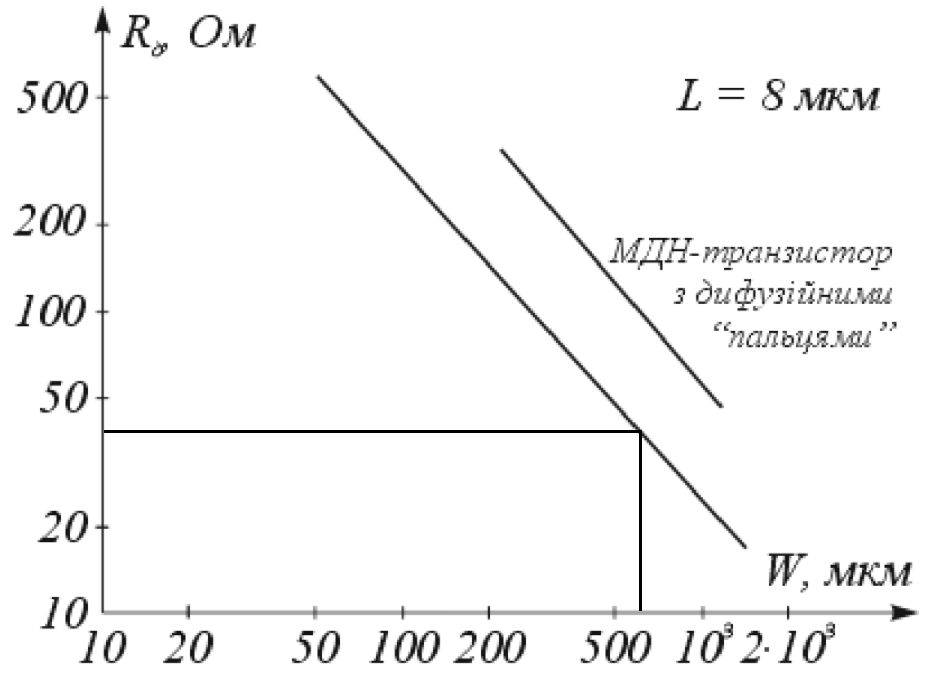
\includegraphics[width=0.8\linewidth]{2-d.png}}
	\caption{Графік для знаходження ширини}
	\label{ris2}
	\end{figure}

	І треба знайти довжину струмообмежуючого опору: $L_{R}=\frac{R_{0} \cdot W_{R}}{\rho_{S}}$, де $W_{R}=5 \text{ мкм}$
	- ширина дифузійної шини, $\rho_{S}=100 \text{ Ом}-$ питомий опір дифузійної шини.
	Тоді
	$$
	\begin{array}{c}
	L_{R}=\dfrac{R_{6} \cdot W_{R}}{\rho_{S}}=750 \text{ мкм} \\

	\end{array}
	$$


	\begin{table}[h]
	\begin{center}

	\caption{ Таблиця розмірів ПЗ для кожного входу}
	\begin{tabular}{|c|c|c|c|c|c|}
	\hline
	& T1   & T2   & T3   & Діод & Резистор \\ \hline
	$W$, \textbackslash{}text\{ мкм\} & 75   & 75   & 75   & 630  & 5        \\ \hline
	L,\textbackslash{}text\{ мкм\}    & 5    & 5    & 5    & 5    & 750      \\ \hline
	$W / L$                           & 6,13 & 6,13 & 6,13 &      &          \\ \hline
	\end{tabular}

	\end{center}
	\end{table}

\newpage
\chapter{ТЕХНОЛОГІЯ ВИГОТОВЛЕННЯ МДН ІС}
	1) Підготовка пластини. Використовується кремній з орієнтацією пластини 111.\\
	2) Перше термічне окиснення кремнієвої пластини товщиною 0,5 мкм. \\
	3) Перша фотолітографія. Розкриття вікон в оксиді в області стоку і витоку. Тип фоторезисту: позитивний, фотошаблон №1, див. Додаток, ДП82.8211.022.001.ФШ, аркуш 1.\\
	4) Дифузія бора, проводиться у дві стадії. Локальна загонка домішки у області стоку і витоку на глибину 1 мкм. Другу стадію виконують в окислювальній атмосфері (друге окислення).\\
	5) Друга фотолітографія. Розкриття вікон під тонкий оксид. Тип фоторезисту: позитивний, фотошаблон №2, \\див. Додаток, ДП82.8211.022.001.ФШ, аркуш 2.\\
	6) Окиснення областей. Вирощення тонкого шару діоксиду силіцію товщиною 50 нм.\\
	7) Підлегування. Іонне підлегування дозою 0,07 мкКл/см$^2$ домішкою фосфору.\\
	8) Третя фотолітографія. Відкриття вікон до областей стоку і витоку. Тип фоторезисту: негативний, фотошаблон №3, див. Додаток, ДП82.8211.022.001.ФШ, аркуш 3.\\
	9) Металізація. Нанесення напиленням плівки алюмінію, товщиною 1,2 мкм, після чого відбувається травлення металу.\\
	10) Четверта фотолітографія. Створення рисунку металізації схеми. Тип фоторезисту: позитивний, фотошаблон №4, див. Додаток, ДП82.8211.022.001.ФШ, аркуш 4.\\
	11) Планаризація і пасивація. Осадження шару фосфорсилікатного скла.\\
	12) П’ята фотолітографія. Відкриття вікна над контактними плолщадками. Тип фоторезисту: негативний, фотошаблон №5, див. Додаток, ДП82.8211.022.001.ФШ, аркуш 5.

\newpage
\chapter{ВИСНОВОК}

\newpage
\chapter{СПИСОК ВИКОРИСТАНОЇ ЛІТЕРАТУРИ }

\newpage
\chapter{ДОДАТОК А }
	\begin{figure}[h!]
	%\center{\includegraphics[width=0.8\linewidth]{A-1.png}}
	\label{ris2-d}
	\end{figure}

\newpage
\chapter{ДОДАТОК Б}
	\begin{landscape}
	\begin{figure}[h!]
	\center{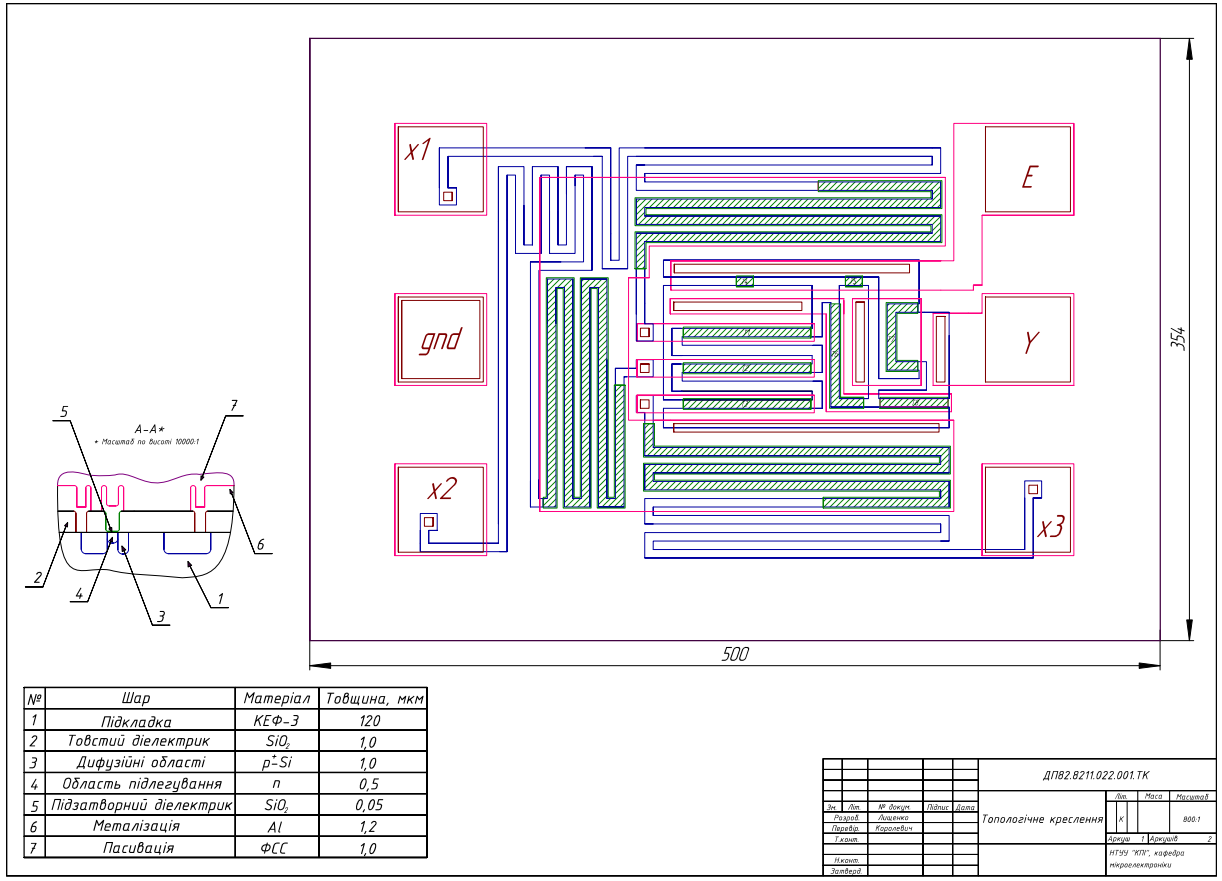
\includegraphics[width=0.9\linewidth]{B-1.png}}

	\label{ris2-d}
	\end{figure}

	\begin{figure}[h!]
	\center{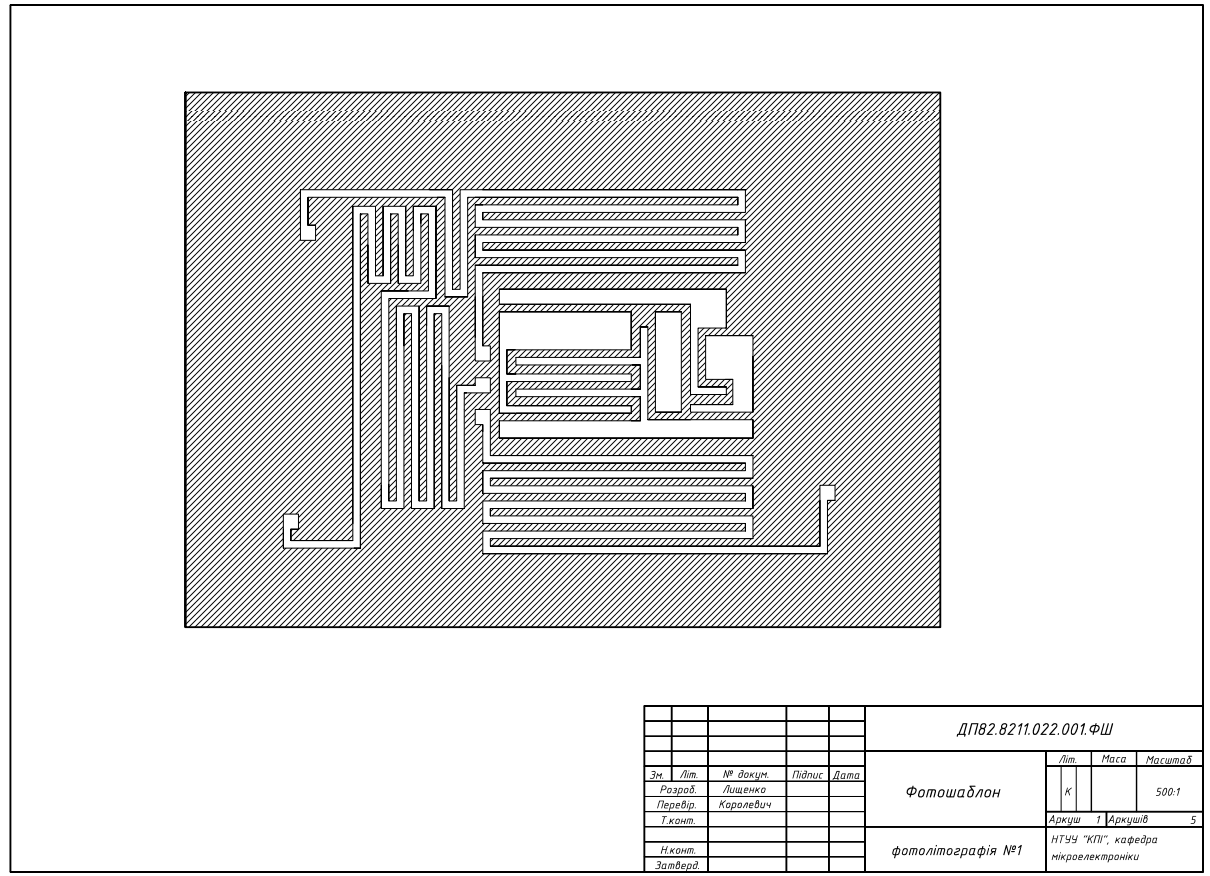
\includegraphics[width=0.9\linewidth]{B-2.png}}

	\label{ris2-d}
	\end{figure}

	\begin{figure}[h!]
	\center{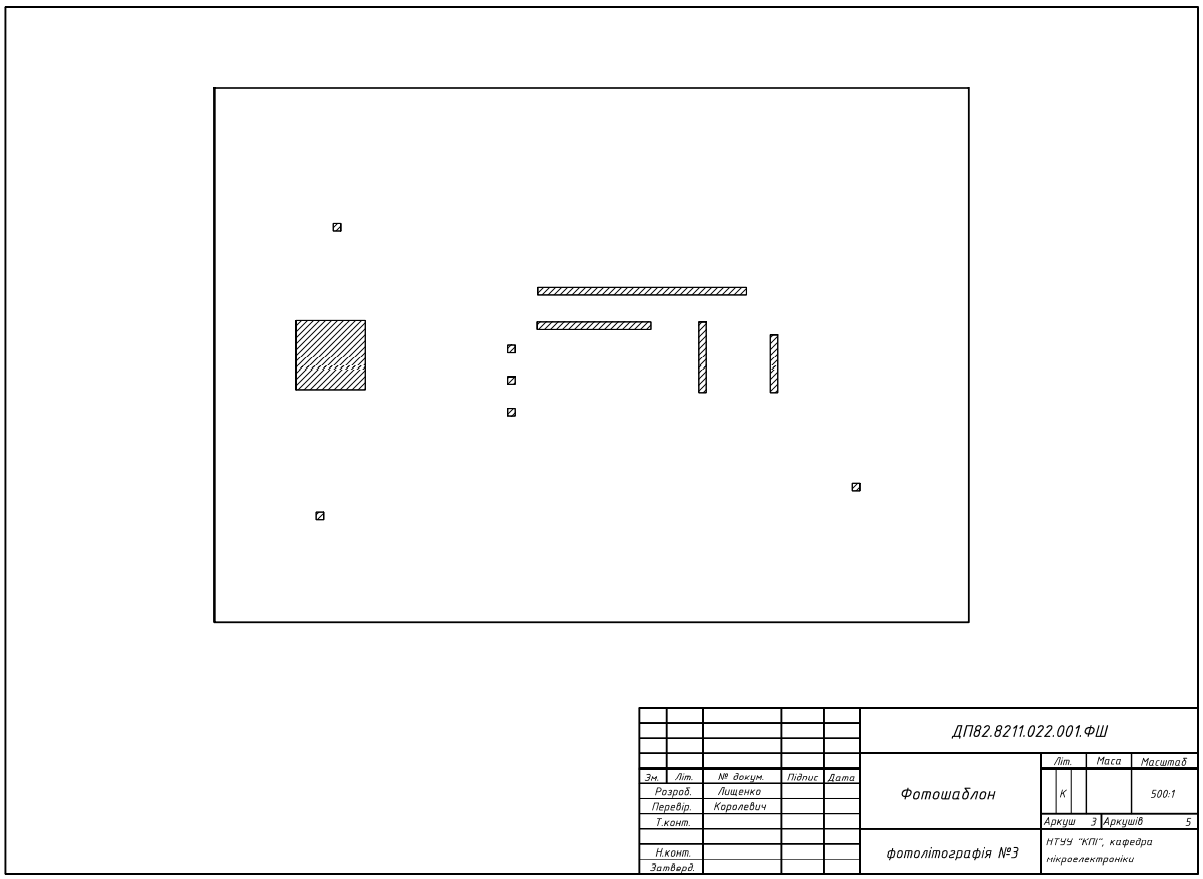
\includegraphics[width=0.9\linewidth]{B-4.png}}

	\label{ris2-d}
	\end{figure}

	\begin{figure}[h!]
	\center{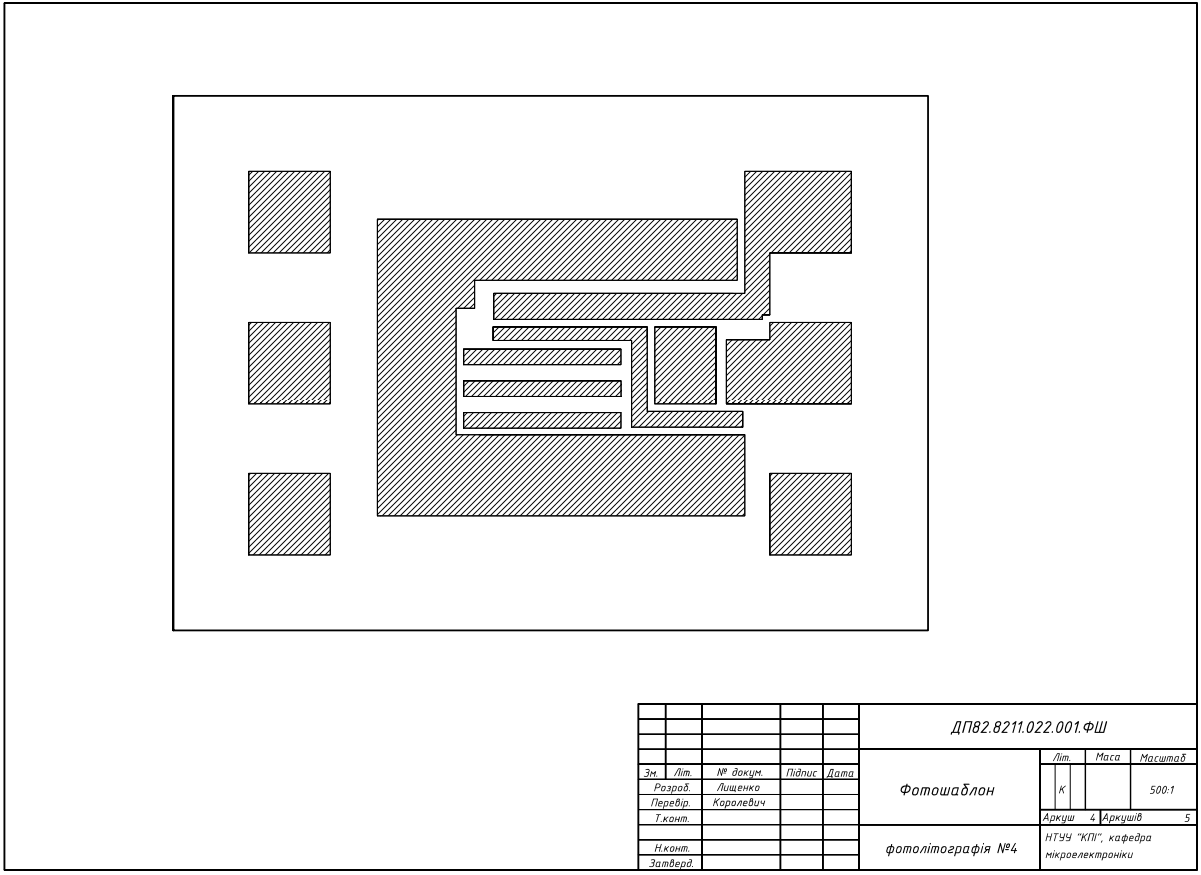
\includegraphics[width=0.9\linewidth]{B-5.png}}

	\label{ris2-d}
	\end{figure}

	\begin{figure}[h!]
	\center{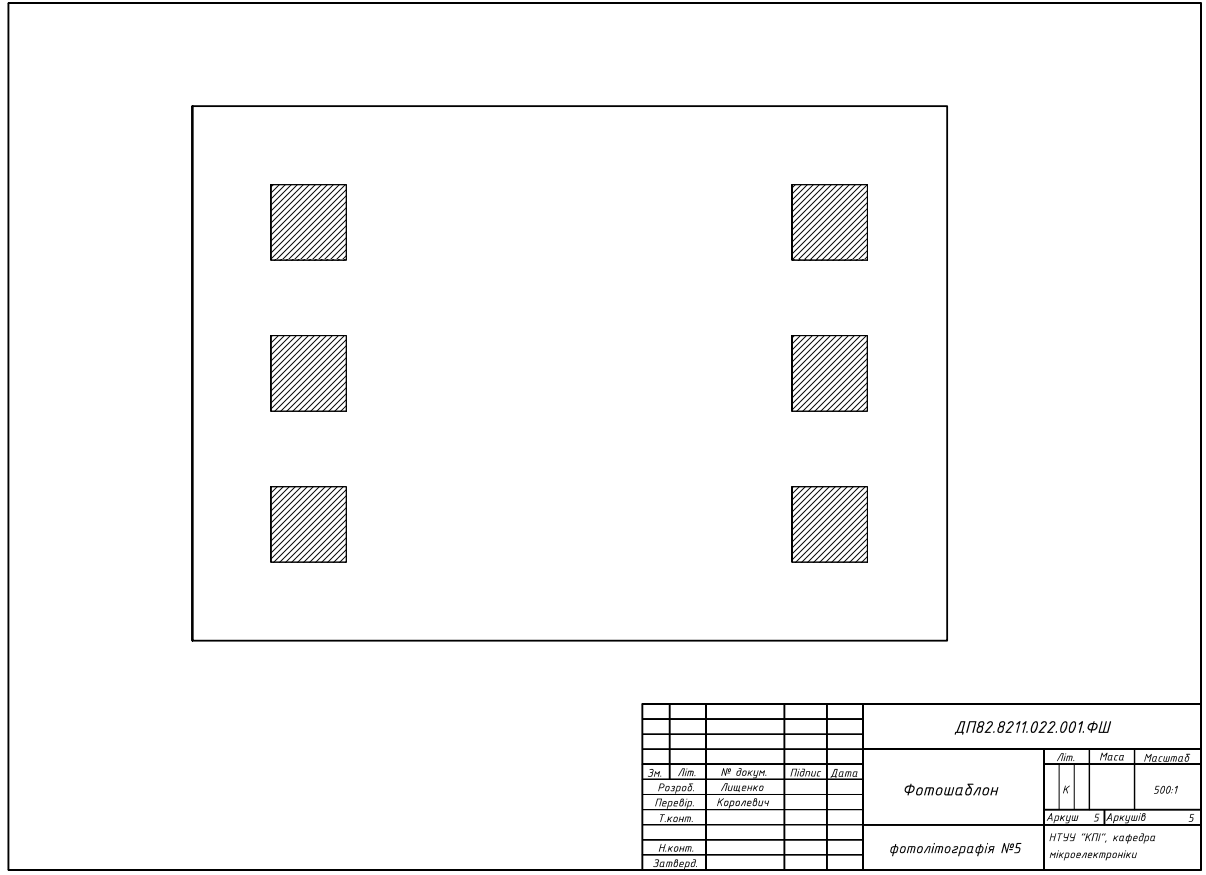
\includegraphics[width=0.9\linewidth]{B-6.png}}

	\label{ris2-d}
	\end{figure}
	\end{landscape}












 
















































\end{document}
